% !TeX program	= xelatex
% !TeX encoding	= UTF-8

%-------------------- 文类 --------------------
\documentclass[UTF8, a4paper, 12pt, oneside, onecolumn]{article}

%-------------------- 宏包 --------------------
\input{../../template/usepackage}
\usepackage[sort, numbers]{natbib}

%-------------------- 杂项 --------------------
\input{../../template/misc}
\def\homeworkName{有限元方法及 Chebyshev 谱方法}
\hypersetup
{
	% 颜色
	colorlinks	= true,
	linkcolor	= black,
	urlcolor	= red,
	citecolor	= black,
	anchorcolor	= blue,
}

%-------------------- 字体设置 --------------------
\input{../../template/fonts}

%-------------------- 标题样式 --------------------
\input{../title}

%-------------------- 自定义符号 --------------------
\input{../../template/symbols}
\newcommand\bH{\mathbb{H}}
\newcommand\bV{\mathbb{V}}
\newcommand\bVh{\mathbb{V}_h}
\newcommand\bVhz{\mathbb{V}_h(0)}
\newcommand\bK{\bm K}
\newcommand\bmf{\bm f}
\newcommand\bv{\bm v}
\newcommand\fT{\mathfrak{T}}
\newcommand\bP{\mathbb{P}}
\newcommand\bmx{\bm x}
\newcommand\whx{\widehat{x}}

%-------------------- 自定义环境 --------------------
\input{../../template/environments}

%-------------------- \item 编号 --------------------
\input{../../template/itemstyle}

%-------------------- 代码样式设置 --------------------
\input{../../template/codestyle}

%-------------------- PDF 元信息, 建模时注释掉 --------------------
\input{../pdfinfo}

%-------------------- 页眉页脚 --------------------
\input{../headersfooters}
\usepackage[ntheorem]{empheq}
\fancypagestyle{plain}{\setboolean{first}{false}	% 在 plain 样式的定义中将 first 重置为 false
\lhead{\songti\zihao{-5} 202121130093\\ 阙嘉豪} \chead{\zihao{-5} 有\quad 限\quad 元\quad 方\quad 法\quad 作\quad 业} \rhead{\zihao{-5} \today}%\monthyeardate\today}
\lfoot{} \cfoot{} \rfoot{}}

%-------------------- 正文 --------------------
\begin{document}

\thispagestyle{plain}

%\columnseprule = 1pt	% 栏线
\begin{center}
	{\zihao{-2}\heiti \homeworkName} \\
	\vspace{1.5ex}
	{\zihao{-4}\fangsong 阙嘉豪\textsuperscript{\hyperref[auth:1]{1}}} \\
	{\zihao{6}\songti \label{auth:1}(1. 北京师范大学 数学科学学院, 北京~~100875)}
\end{center}

\zihao{5}

%\watermark{60}{10}{\currenttime}

\section{模型问题}

考虑 $\Omega := (0, 1)^2$ 上的 Poisson 方程的 Dirichlet 边值问题:
\begin{subequations}\label{equ:DirichletProblem}
\begin{align}
	-\D u &= \dfrac{1}{\(\a + r\)} \l[
		- \dfrac{\cos \(\dfrac{1}{\a + r}\)}{r}
		+ \dfrac{2 \cos \(\dfrac{1}{\a + r}\)}{\(\a + r\)^2}
		- \dfrac{\sin \(\dfrac{1}{\a + r}\)}{\(\a + r\)^3}
	\r],\quad (x, y) \in (0, 1)^2,\\
	u(x, y) &= \lb\begin{array}{ll}
		\sin\(\dfrac{1}{\a + x}\),	&	(x, y) \in [0, 1] \times \lrb{0},\\
		\sin\(\dfrac{1}{\a + \sqrt{1 + y^2}}\),	&	(x, y) \in \lrb{1} \times [0, 1],\\
		\sin\(\dfrac{1}{\a + \sqrt{x^2 + 1}}\),	&	(x, y) \in [0, 1] \times \lrb{1},\\
		\sin\(\dfrac{1}{\a + y}\),	&	(x, y) \in \lrb{0} \times [0, 1],\\
	\end{array}\rd
\end{align}
\end{subequations}
其中 $\a$ 分别取 0.05 和 0.005. 真解 $u(x, y) = \sin\(\dfrac{1}{\a + r}\)$.

\section{Galerkin 方法}

问题 \eqref{equ:DirichletProblem} 相应于虚功原理的弱解的提法为
\begin{equation}\label{equ:VirtWorkPrince}
	\lb \begin{aligned}
		\text{求}~u &\in \bH_0^1 (\Omega ),\quad \text{使得}\\
		a(u, v) &= (f, v),\quad \forall v \in \bH_0^1 (\Omega ),
	\end{aligned} \rd
\end{equation}
其中
$$a(u, v) = \dint_\Omega \nabla u \cdot \nabla v \di \bm x,\quad (f, v) = \dint_\Omega fv \di \bm x.$$
通常将问题 \eqref{equ:VirtWorkPrince} 的允许函数空间称为试探函数空间.

为了数值求解问题 \eqref{equ:VirtWorkPrince}, 我们给出一个有限维的子空间 $\bV_h(0) \subset \bH_0^1(\Omega )$, 将问题的试探函数空间和检验函数空间分别换成其子空间 $\bV_h(0) \subset \bH_0^1 (\Omega )$, 就给出了该问题相应的近似解的提法:
\begin{equation}\label{equ:ApproxSolution}
	\lb \begin{aligned}
		\text{求}~u_h &\in \bV_h (0),\quad \text{使得}\\
		a(u_h, v_h) &= (f, v_h),\quad \forall v_h \in \bV_h (0).
	\end{aligned} \rd
\end{equation}
通常将该提法称为 Glaerkin 方法, 下面将其化为线性代数方程组求解.

设 $\lrb{\p_i}_{i = 1}^{N_h}$ 是 $\bV_h(0)$ 的一组基, 令
\begin{equation*}
	u_h = \dsum_{j = 1}^{N_h} u_j\p_j,\quad v_h = \dsum_{i = 1}^{N_h} v_i \p_i,
\end{equation*}
则离散问题 \eqref{equ:ApproxSolution} 等价于
\begin{equation*}
	\lb \begin{aligned}
		\text{求}~\bu_h &= \(u_1, \cdots, u_{N_h}\)^\T \in \R^{N_h},\quad \text{使得}\\
		\dsum_{i, j = 1}^{N_h} a\(\p_j, \p_i\) u_jv_i &= \dsum_{i = 1}^{N_h} \( f, \p_i \) v_i,\quad \forall \bv_h = \(v_1, \cdots, v_{N_h}\)^\T \in \R^{N_h}.
	\end{aligned} \rd
\end{equation*}
由 $\bv_h$ 的任意性, 这等价于求解线性代数方程组
\begin{equation}\label{equ:LinAlgEqus}
	\dsum_{j = 1}^{N_h} a\(\p_j, \p_i\) u_j = \( f, \p_i \),\quad i = 1, \cdots, N_h.
\end{equation}
通常将线性代数方程组 \eqref{equ:LinAlgEqus} 写为矩阵形式
\begin{equation}\label{equ:Kuhf}
	\bm K \bu_h = \bm f,
\end{equation}
称 $\bm K := \(k_{ij}\) := \(a\( \p_j, \p_i \)\)$ 为刚度矩阵, $\bu_h$ 为位移向量, $\bmf := \(f_i\) := \(\(f, \p_i\)\)$ 为载荷向量. 由 $a\(\cdot, \cdot\)$ 的对称性和 Poincar\'{e}-Friedrichs 不等式, 容易证明刚度矩阵 $\bK$ 是对称正定矩阵. 由此也可以证明线性代数方程组 \eqref{equ:LinAlgEqus} 的解的存在唯一性.

\section{有限元方法}

下面构造有限维的子空间 $\bV_h(0) \subset \bH_0^1 (\Omega )$ 以及选取 $\bV_h(0)$ 上的一组基, 并给出刚度矩阵和载荷向量的求解方法.

\subsection{三角形剖分}

对 $\ol{\Omega}$ 做如图 \ref{fig:triangle_grid} 所示的三角形剖分 $\fT_h(\Omega)$, 即将其分割为 $M = 2L^2$ 个互相之间没有公共内点的三角形单元 $T_i$, $i = 1, \cdots, M$, 其中参数 $h := \underset{1 \leq i \leq M}{\max } \dsup_{x, y \in T_i} \lrvv{x - y}$ 是剖分中所有单元的最大直径. 将剖分的 $N = (L + 1)^2$ 个节点作整体编号 $A_i$, $i = 1, \cdots, N$, 公共的节点共用一个整体编号, 并将节点分为边界节点和内部节点两类.

\usetikzlibrary{math}
\begin{figure}[H]\centering\zihao{-5}
	\begin{tikzpicture}
		\tikzmath{
			int \L, \Tname1, \Tname2;
			\L = 4;
		}
		\foreach \x in {1, ..., \L}
		{
			\foreach \y in {1, ..., \L}
			{
				\draw (\x, \y) +(-.5, -.5) rectangle ++(.5, .5);
				\draw (\x, \y) +(-.5, .5) -- ++(.5, -.5);
				\tikzmath{
					\Tname1 = 2 * (\L * (\y - 1) + \x) - 1;
					\Tname2 = 2 * (\L * (\y - 1) + \x);
				}
				\draw (\x, \y) +(-.2, -.2) node{$T_{\Tname1}$};
				\draw (\x, \y) +(.2, .2) node{$T_{\Tname2}$};
			}
		}
		\tikzmath{
			\L = \L + 1;
		}
		\foreach \x in {1, ..., \L}
		{
			\foreach \y in {1, ..., \L}
			{
				\tikzmath{
					\Tname1 = \L * (\y - 1) + \x;
				}
				\draw (\x, \y) +(-.65, -.65) node{\zihao{-6} $\Tname1$};
			}
		}
	\end{tikzpicture}
	\caption{$L = 4$ 时的三角形剖分}\label{fig:triangle_grid}
\end{figure}

\subsection{有限元函数空间}	% \texorpdfstring{$\bV_h(0)$}{V\_h(0)}

在三角形剖分 $\fT_h(\Omega )$ 的基础上定义有限元函数空间
\begin{equation*}
	\bV_h := \lrb{u \in C\(\ol{\Omega}\) : u|_{T_i} \in \bP_1\(T_i\), \forall T_i \in \fT_h(\Omega )},
\end{equation*}
并根据齐次强制边界条件取有限元试探函数空间和检验函数空间为
\begin{equation*}
	\bV_h(0) := \lrb{u \in \bV_h : u\(A_i \) = 0, \forall A_i \in \pa \Omega},
\end{equation*}
其中 $\bP_k\(T_i \)$ 表示定义在 $T_i$ 上的所有次数不超过 $k$ 的多项式所构成的线性空间. $\bV_h$ 是 $\bH^1(\Omega )$ 的子空间, $\bV_h(0)$ 是 $\bH_0^1(\Omega )$ 的子空间.

\subsection{单元基底函数}

由于 $\bV_h$ 和 $\bV_h(0)$ 都是由分片线性的连续函数构成的, 易证 $\bV_h$ 和 $\bV_h(0)$ 中的任意一个函数都由其节点函数值 $\lrb{u\( A_i \)}_{i = 1}^N$ 唯一确定. 设 $\p_i \in \bV_h$ 满足
$$\p_i\(A_i\) = \de_{ij},\quad i = 1, \cdots, N,$$
则 $\lrb{\p_i}_{i = 1}^N$ 组成了 $\bVh$ 的一组基, 而 $\lrb{\p_i}_{A_i \notin \pa \Omega}$ 组成了 $\bVhz$ 的一组基.

\begin{Remark}
	上述有限元函数空间的基底函数的支集很小, 由有限元方法得到的刚度矩阵为稀疏矩阵, 其零元素的分布依赖于节点的排序. 尽管排序并不影响解的性质, 但适当的节点排序有利于提高数值求解线性代数方程的效率.
\end{Remark}

\subsection{单元刚度矩阵和单元载荷向量}

建立了有限元函数空间 $\bVhz$ 后, 我们就可以计算刚度矩阵 $\bK$ 和载荷向量 $\bmf$. 首先需要计算单元刚度矩阵和单元载荷向量, 然后进行组装. 为了便于数据管理, 引入以下两个数组:
\begin{itemize}
	\item $en(\a, e)$: 第 $e$ 个单元的第 $\a$ 个节点对应于第 $en(\a, e)$ 个整体节点;
	\item $cd(i, nd)$: 第 $nd$ 个整体节点的空间坐标的第 $i$ 个分量.
\end{itemize}
记
$$a^e(u, v) := \dint_{T_e} \nabla u \cdot \nabla v \di \bmx,$$
由定义有
$$k_{ij} := a\(\p_j, \p_i\) = \dsum_{e = 1}^M a^e\(\p_j, \p_i\) = \dsum_{e = 1}^M \dint_{T_e} \nabla \p_j \cdot \nabla \p_i \di \bmx = \dsum_{e = 1}^M k_{ij}^e.$$
由于有大量的 $k_{ij}$ 为零, 而且即便 $k_{ij} \neq 0$, 上式的几个求和式中也只有少数几项非零, 并且只有 $i$, $j$ 两个节点同属一个单元 $T_e$ 时 $\dint_{T_e} \nabla \p_j \cdot \nabla \p_i \di \bmx \neq 0$. 因此通常不采取扫描节点 $i$, $j$ 的方式计算 $k_{ij}$ 而是通过扫描单元的方式计算.

对于每一个单元 $T_e$ 定义单元刚度矩阵
$$\bK^e := \(k_{\a\ba}^e\),\quad k_{\a\ba}^e := a^e\(\p_\a^e, \p_\ba^e\) = \dint_{T_e} \nabla \p_\a^e \cdot \nabla \p_\ba^e \di \bmx,$$
则有
$$k_{ij} = \dsum_{\substack{en(\a, e) = i \in T_e\\ en(\ba, e) = j \in T_e}} k_{\a\ba}^e.$$
同理也可以通过扫描单元来计算载荷向量 $\bmf := \(f_i\)$:
$$f_i = \dsum_{en(\a, e) = i \in T_e} \dint_{T_e} f\lambda_\a^e \di \bmx =: \dsum_{en(\a, e) = i \in T_e} f_\a^e.$$
我们称 $\bmf := \(f_\a^e\)$ 为单元载荷向量.

下面通过变量替换将单元刚度矩阵和单元载荷向量的计算转化到标准三角形上.

设 $\a = 1, 2, 3$ 为 $T_e$ 的三个节点 $A_i$, $A_j$, $A_k$ 的局部节点序数, 即在单元 $T_e$ 上这三个节点分别记作 $A^e_1$, $A^e_2$ 和 $A^e_3$. 设 $\lambda_\a^e \in \bP_1\(T_e\)$ 满足 $\lambda_\a^e\(A_\ba^e\) = \de_{\a\ba}$, 则有
$$\lambda_\a^e(A) = \dfrac{\lrv{\nabla AA_\ba^e A_\gamma^e}}{\lrv{\nabla A_\a^e A_\ba^e A_\gamma^e}},\quad \forall A \in T_e,$$
其中 $\lrv{T}$ 为集合 $T$ 的面积. 通常称 $\lambda^e(A) := \(A^e_1(A), A^e_2(A), A^e_3(A)\)^\T$ 为 $A \in T_e$ 的面积坐标. 易证 $\lambda_\a^e = \p_{en(\a, e)}|_{T_e}$, 且 $\lrb{\lambda_\a^e}_{\a = 1}^3$ 为 $\bP_1\(T_e \)$ 的一组基. 事实上, 对任意 $u \in \bP_1\(T_e\)$, 有
$$u(A) = \dsum_{\a = 1}^3 u\(A_\a^e\) \lambda_\a^e(A),\quad \forall A \in T_e.$$

所有的单元 $T_e$ 都与标准三角形
$$T_s := \lrb{\wh{\bmx} = \(\whx_1, \whx_2\) \in \R^2 : \whx_1 \geq 0, \whx_2 \geq 0, \whx_1 + \whx_2 \leq 1}$$
仿射等价, 即对任意的三角形单元 $T_e$, 存在可逆矩阵 $\bm A_e \in \R^{2 \times 2}$ 和向量 $\bm a_e$, 使得仿射变换
$$\bmx = L_e\(\wh{\bmx}\) := \bm A_e\wh{\bmx} + \bm a_e$$
将 $T_s$ 映射到 $T_e$. 同时仿射变换 $L_e\(\wh{\bmx}\)$ 也诱导了 $\bP_1\(T_s\)$ 和  $\bP_1\(T_e\)$ 之间的一个一一对应关系. 将 $T_s$ 的三个顶点坐标记为
$$\bm A^s_1 = (0, 0)^\T,\quad \bm A^s_2 = (1, 0)^\T,\quad \bm A^s_3 = (0, 1)^\T,$$
容易得到 $T_s$ 的面积坐标为
$$\lambda^s_1\(\whx_1, \whx_2\) = 1 - \whx_1 - \whx_2,\quad \lambda^s_2\(\whx_1, \whx_2\) = \whx_1,\quad \lambda^s_3 \(\whx_1, \whx_2\) = \whx_2.$$
若 $T_e$ 的三个顶点的坐标为
$$\bm A^e_1 = (x^1_1, x^1_2)^\T,\quad \bm A^e_2 = (x^2_1, x^2_2)^\T,\quad \bm A^e_3 = (x^3_1, x^3_2)^\T,$$
则有
$$\bm A_e = \(\bm A^e_2 - \bm A^e_1, \bm A^e_3 - \bm A^e_1\),\quad \bm a_e = \bm A^e_1.$$
由 $\lambda_\a^s \(L_e^{-1} (\bm x)\)$ 是 $\bmx$ 的线性函数及 $\lambda_\a^s\( L_e^{-1}\( \bm A_\ba^e \) \) = \lambda_\a^s\(\bm A_\ba^s \) = \de_{\a\ba}$ 知, $T_e$ 的面积坐标可以用 $T_s$ 的面积坐标表示为 $\lambda_\a^e\(\bm x\) = \lambda_\a^s \( L_e^{-1}\( \bm A_\ba^e \) \)$. 由此得
\begin{align*}
	\wh{\bmx} &= L_e^{-1}\(\wh{\bmx}\) = \bm A_e^{-1} \bmx - \bm A_e^{-1} \bm A_1^e, \\
	\nabla \lambda^e(\bmx) &= \nabla \lambda^s \(\wh{\bmx}\) \nabla L_e^{-1} (\bmx) = \nabla \lambda^s\(\wh{\bmx}\) \bm A_e^{-1}.
\end{align*}
因此, 可以将单元刚度矩阵 $\bK^e$ 和单元载荷向量 $\bmf$ 的计算统一在标准三角形 $T_s$ 上进行, 即
\begin{align*}
	\bK^e &= \dint_{T_e} \nabla \lambda^e(\bmx) \(\nabla \lambda^e(\bmx)\)^\T \di \bmx\\
	&= \dint_{T_s} \nabla \lambda^s(\wh{\bmx}) \bm A_e^{-1} \(\nabla \lambda^s(\wh{\bmx}) \bm A_e^{-1}\)^\T \det \bm A_e \di \wh{\bmx}.
\end{align*}
由此及
$$\nabla \lambda^s\( \wh{\bmx} \) = \begin{pmatrix}
	-1 & -1\\
	1 & 0\\
	0 & 1
\end{pmatrix},\quad \bm A_e^{-1} = \dfrac{1}{\det \bm A_e} \begin{pmatrix}
	x_2^3 - x_2^1	&	x_1^1 - x_1^3\\
	x_2^1 - x_2^2	&	x_1^2 - x_1^1
\end{pmatrix}$$
并注意到 $T_s$ 的面积为 $\dfrac{1}{2}$, 就立即得到单元刚度矩阵为
$$\bK^e = \dfrac{1}{2\det \bm A_e} \begin{pmatrix}
	x_2^2 - x_2^3	&	x_1^3 - x_1^2\\
	x_2^3 - x_2^1	&	x_1^1 - x_1^3\\
	x_2^1 - x_2^2	&	x_1^2 - x_1^1
\end{pmatrix} \begin{pmatrix}
	x_2^2 - x_2^3	&	x_2^3 - x_2^1	&	x_2^1 - x_2^2\\
	x_1^3 - x_1^2	&	x_1^1 - x_1^3	&	x_1^2 - x_1^1
\end{pmatrix}.$$
类似地可以得到单元载荷向量的计算公式
\begin{equation}\label{equ:bmfe}
	\bmf^e = \dint_{T_e} f(\bmx) \lambda^e(\bmx) \di \bmx = \det \bm A_e \dint_{T_s} f\( L_e\( \wh{\bmx} \) \) \lambda^s \(\wh{\bmx}\) \di \wh{\bmx}.
\end{equation}
一般地, 单元载荷向量的计算要用到数值积分公式. 不过, 当 $f$ 为分片多项式时, 可以通过 \eqref{equ:bmfe} 式右端的积分给出直接的计算公式. 例如, $f$ 在 $T_e$ 上为常数时, 有
$$\bmf^e = \dfrac{1}{6} f\(T_e\) \det \bm A_e \(1, 1, 1\)^\T = \dfrac{1}{3} f\(T_e\)\lrv{T_e} \(1, 1, 1\)^\T,$$
其中 $\lrv{T_e}$ 为 $T_e$ 的面积. 而 $f$ 为分片线性时, 设 $f|_{T_e} = \dsum_{i = 1}^3 f_i^e\lambda_i^e(\bmx)$, 有
$$\bmf^e = \dfrac{\lrv{T_e}}{12}\begin{pmatrix}
	2 & 1 & 1\\
	1 & 2 & 1\\
	1 & 1 & 2
\end{pmatrix} \begin{pmatrix}
	f_1^e\\
	f_2^e\\
	f_3^e
\end{pmatrix}.$$
至此, 我们完成了单元刚度矩阵和单元载荷向量的计算.

\subsection{组装刚度矩阵和载荷向量}

下面组装刚度矩阵和载荷向量, 算法如下.

\begin{algorithm}[H]
	\caption{形成刚度矩阵和载荷向量的算法}\label{alg:con_stiff_mat_and_load_vec}
	\zihao{-5}
	\begin{algorithmic}[1]
		% \Require 直杆影子端点坐标 $\(x_i^*, y_i^*\), i = 1, 2, \cdots, n$.
		% \Ensure 纬度 $\phi$, 经度 $\psi$.
		\State {$\bK = \(k(i, j)\) \gets 0$, $\bmf = \(f(i)\) \gets 0$.}
		\For {$e$}{$1$}{$M$}
			\State {计算单元刚度矩阵 $\bK^e = \(k^e(\a, \ba)\)$.}
			\State {计算单元载荷向量 $\bmf^e = \(f^e(\a)\)$.}
			\State {$k\(en(\a, e), en(\ba, e)\) \gets k\(en(\a, e), en(\ba, e)\) + k^e(\a, \ba)$.}
			\State {$f\(en(\a, e)\) \gets f\(en(\a, e)\) + f^e(\a)$.}
		\EndFor
	\end{algorithmic}
\end{algorithm}

由单元刚度矩阵和单元载荷向量得到总的刚度矩阵和载荷向量, 便可根据 \eqref{equ:Kuhf} 式建立与原问题等价的有限元离散线性代数方程组, 简称有限元方程.

% \subsection{相容性}

% \subsection{稳定性}

% \subsection{收敛性}

% \subsection{误差分析}

\section{数值实验}

% 在问题 \eqref{equ:DirichletProblem} 中取
% $$f(x, y) := -2\(x(x - 1) + y(y - 1)\),$$
% 对应的解析解为
% $$u(x, y) = x(x - 1)y(y - 1).$$
% f = (x, y) -> -2.0 * (x^2 + y^2 - x - y),
% u = (x, y) -> x * (x - 1) * y * (y - 1),

问题 \eqref{equ:DirichletProblem} 中取 $\a = 0.05$, $\a = 0.005$ 时不同单元直径的 $\mathbb{H}^1$ 误差及收敛阶如表 \ref{tab:errorNormalpha0.05} 所示. 可以看出, 随着 $h$ 的减小, 误差的 $\mathbb{H}^1$ 范数逐渐减小, $\a = 0.05$ 时收敛阶逐渐接近于 $2$. $\alpha = 0.005$ 时真解较为病态, 收敛缓慢.

\begin{figure}[H]\centering
	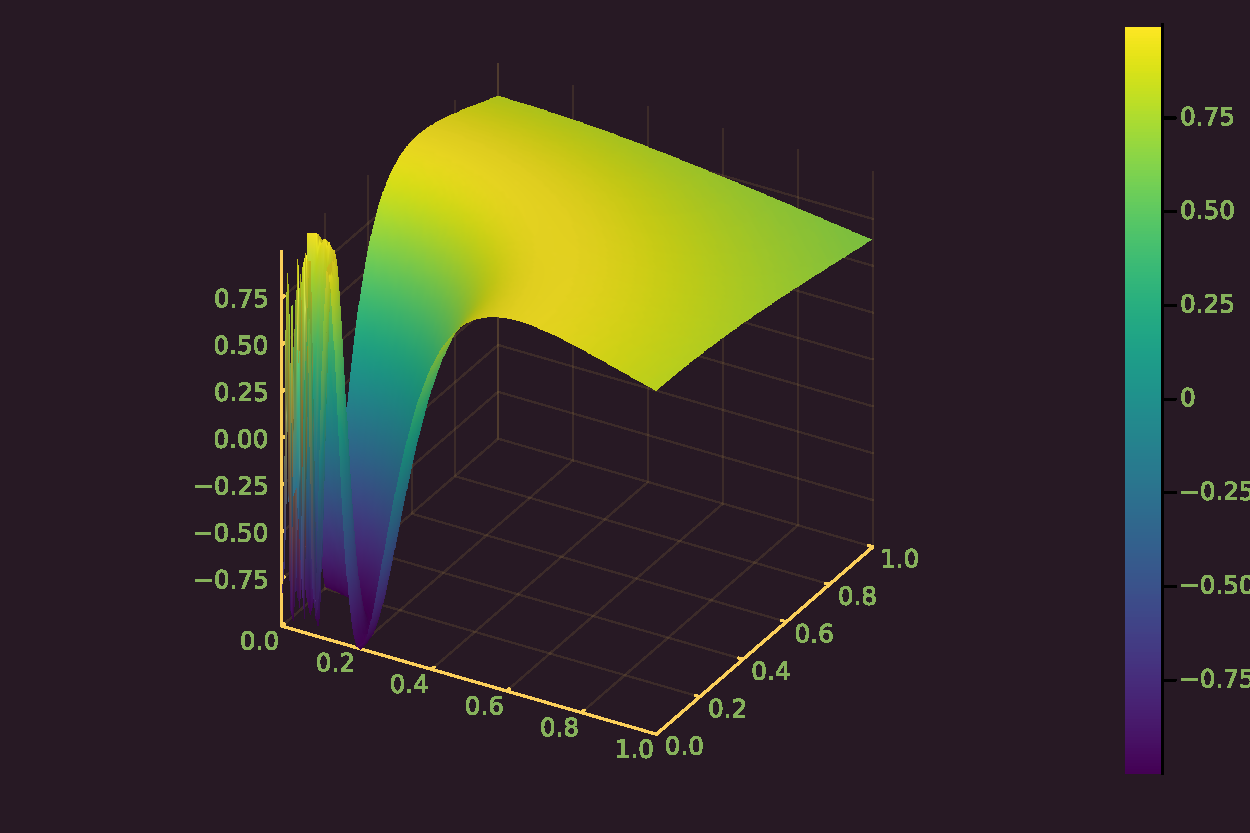
\includegraphics[width=.48\linewidth]{2du_alpha.pdf}~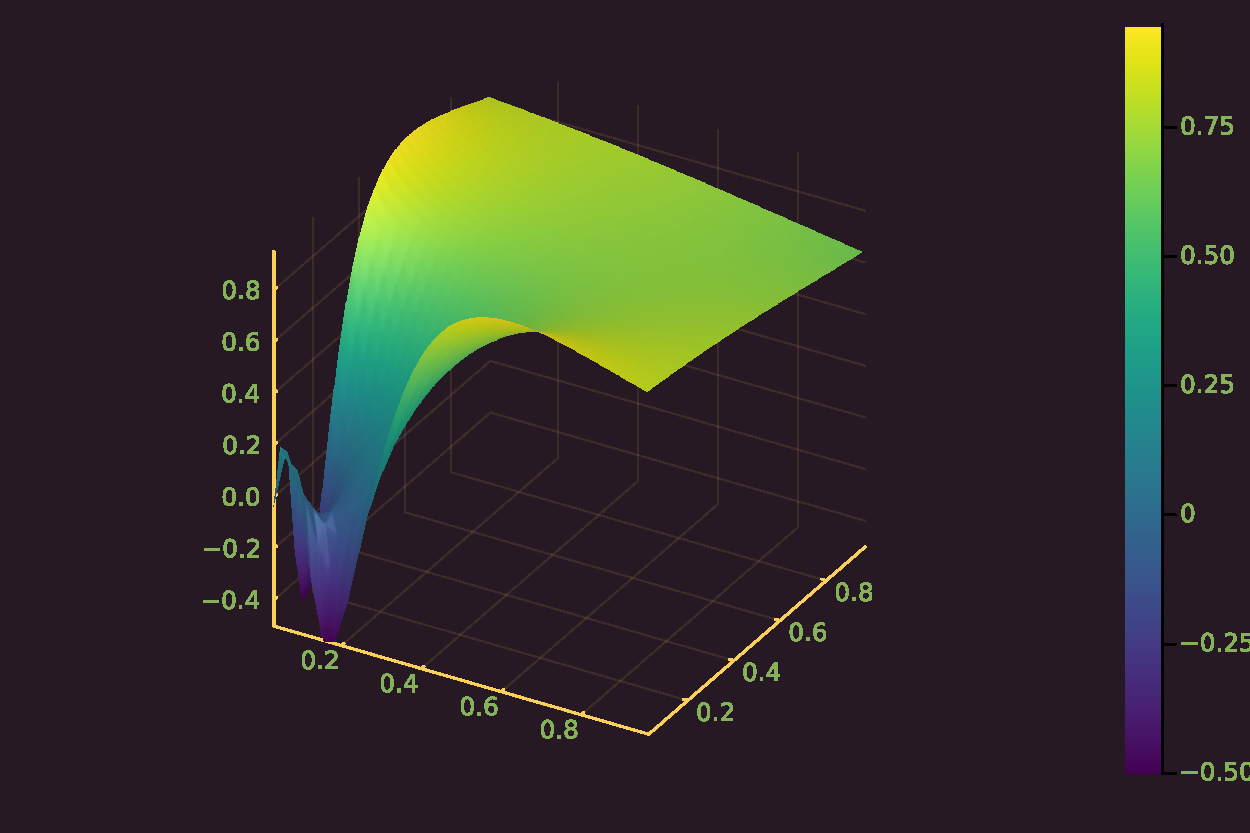
\includegraphics[width=.48\linewidth]{2du_alpha0005.pdf}
	\caption{$\a = 0.05$ 及 $\a = 0.005$ 时的解}\label{fig:2dFEMalpha}
\end{figure}

\begin{table}[H]\centering\heiti\zihao{-5}
	\caption{$\a = 0.05$ 不同单元直径时的 $\mathbb{H}^1$ 误差及收敛阶}\label{tab:errorNormalpha0.05}
	\begin{tabular}{|c|c|c|c|}\hline
		$h$ &   $\lrv{u-u_h}_{\mathbb{H}^1}$ &   收敛阶  &   运行时间 (秒)\\\hline
		% $2^{-2}$	&	$0.0847761$	&		&	$0.414929$\\\hline
		$2^{-3}$	&	$0.0629238$	&	$0.43005$	&	$0.00290608$\\\hline
		$2^{-4}$	&	$0.0266285$	&	$1.24064$	&	$0.00477099$\\\hline
		$2^{-5}$	&	$0.0105705$	&	$1.33293$	&	$0.0128319$\\\hline
		$2^{-6}$	&	$0.00361737$	&	$1.54703$	&	$0.045805$\\\hline
		$2^{-7}$	&	$0.00111925$	&	$1.69241$	&	$0.226058$\\\hline
		$2^{-8}$	&	$0.000317549$	&	$1.81748$	&	$0.913255$\\\hline
		$2^{-9}$	&	$0.0000841953$	&	$1.91517$	&	$3.24802$\\\hline
		$2^{-10}$	&	$0.0000217025$	&	$1.95588$	&	$14.766$\\\hline
		$2^{-11}$	&	$0.00000551374$	&	$1.97676$	&	$62.6182$\\\hline
	\end{tabular}
\end{table}

\begin{table}[H]\centering\heiti\zihao{-5}
	\caption{$\a = 0.005$ 不同单元直径时的 $\mathbb{H}^1$ 误差及收敛阶}\label{tab:errorNormalpha0.005}
	\begin{tabular}{|c|c|c|c|}
		\hline
		$h$ &   $\lrv{u-u_h}_{\mathbb{H}^1}$ &   收敛阶  &   运行时间 (秒)\\\hline
		% $2^{-2}$	&	$0.106428$	&		&	$0.421079$\\\hline
		$2^{-3}$	&	$0.11268$	&	$-0.0823514$	&	$0.00288391$\\\hline
		$2^{-4}$	&	$0.0621768$	&	$0.857786$	&	$0.00464201$\\\hline
		$2^{-5}$	&	$0.051414$	&	$0.274217$	&	$0.0119009$\\\hline
		$2^{-6}$	&	$0.0240167$	&	$1.09812$	&	$0.0427032$\\\hline
		$2^{-7}$	&	$0.0082512$	&	$1.54136$	&	$0.222058$\\\hline
		$2^{-8}$	&	$0.00357763$	&	$1.2056$	&	$1.08011$\\\hline
		$2^{-9}$	&	$0.00148462$	&	$1.26891$	&	$4.04617$\\\hline
		$2^{-10}$	&	$0.000297185$	&	$2.32066$	&	$17.4789$\\\hline
		$2^{-11}$	&	$0.0000542527$	&	$2.45359$	&	$66.5752$\\\hline
	\end{tabular}
\end{table}

\section{Chebyshev 谱方法}

由 \cite{Gottlieb1984TheoryAA}, Chebyshev 网格点:
\begin{equation}
	x_i=\cos \left(\frac{\pi i}{N}\right), \quad i=0, \ldots, N.
\end{equation}
基函数:
\begin{subequations}
\begin{align}
	C_j(x) & \equiv(-1)^{j+1} \frac{\left(1-x^2\right)}{c_j N^2\left(x-x_j\right)} \frac{\di T_N(x)}{\di x} \\
	&=\frac{2}{N p_j} \sum_{m=0}^N \frac{1}{p_m} T_m\left(x_j\right) T_m(x),
\end{align}
\end{subequations}
其中若 $j = 0$ 或 $N$, 则 $p_j = 2$, 若 $j = 1, \cdots, N - 1$, 则 $p_j = 1$, 若 $\lrv{j} < N$, 则 $c_j = 1$, $c_{\pm N} = 2$.
其一阶导数为
\begin{equation}
	D_{ij} = \left.\frac{\di C_j}{\di x}\right|_{x=x_i}=\left\{\begin{array}{cl}
	\dfrac{1+2 N^2}{6}, & i=j=0, \\
	-\dfrac{1+2 N^2}{6}, & i=j=N, \\
	-\dfrac{x_j}{2\left(1-x_j^2\right)}, & i=j, 0<j<N, \\
	\dfrac{(-1)^{i+j} p_i}{p_j\left(x_i-x_j\right)}, & i \neq j.
	\end{array}\right.
\end{equation}
对于问题
\begin{subequations}\label{equ:sinx}
	\begin{align}
		-u'' + u &= 2\sin x,\quad x \in (0, \pi),\\
		u(0) = u(\pi) &= 0,
	\end{align}
\end{subequations}
真解为 $u = \sin x$, 对其进行离散得到
\begin{equation*}
	(- D^2 + I) U = F,
\end{equation*}
其中 $F_{i} = -2\sin x_i$.

分别使用有限元方法和 Chebyshev 谱方法求解问题 \eqref{equ:sinx}, 得到结果如图 \ref{fig:1dFEMSM3}, \ref{fig:1dFEMSM} 和表 \ref{tab:1dFEMSM} 所示.

由表 \ref{tab:1dFEMSM} 可以看出 Chebyshev 谱方法收敛速度较快, 网格较小时运行较快, 但网格较大时, 因其系数矩阵为稠密矩阵, 故求解速度较慢. 而有限元方法收敛较慢, 优点是矩阵稀疏, 求解速度较快.

\newgeometry{left = 2.18 cm, right = 2.18 cm}

\begin{figure}[H]\centering
	\includegraphics[width=.48\linewidth]{1dFEM3.pdf}~\includegraphics[width=.48\linewidth]{1dSM3.pdf}
	\caption{$h = 2^{-3}\pi$ 时有限元方法及 Chebyshev 谱方法的解}\label{fig:1dFEMSM3}
\end{figure}

\begin{figure}[H]\centering
	\includegraphics[width=.48\linewidth]{1dFEM.pdf}~\includegraphics[width=.48\linewidth]{1dSM.pdf}
	\caption{$h = 2^{-5}\pi$ 时有限元方法及 Chebyshev 谱方法的解}\label{fig:1dFEMSM}
\end{figure}

\begin{table}[H]\centering\heiti\zihao{-5}
	\caption{不同单元直径及 Chebyshev 点数量 $N = \dfrac{\pi}{h}$ 时的 $\mathbb{H}^1$ 误差及收敛阶}\label{tab:1dFEMSM}
	\begin{tabular}{|c|c|c|c|c|c|c|}
		\hline
		$h$	&	有限元 $\lrvv{u - u_h}_{\mathbb{H}^1}$	&	收敛阶	&	运行时间 (秒)	&	谱方法 $\lrvv{u - u_h}_{\mathbb{H}^1}$	&	收敛阶	&	运行时间 (秒)\\\hline
		$2^{-2}\pi$	&	$0.0389822$	&		&	$0.528757$	&	$0.0274445$	&		&	$0.608137$\\\hline
		$2^{-3}\pi$	&	$0.00816688$	&	$2.25496$	&	$9.70364 \times 10^{-5}$	&	$3.88296 \times 10^{-6}$	&	$12.7871$	&	$4.50611 \times 10^{-5}$\\\hline
		$2^{-4}\pi$	&	$0.00181701$	&	$2.16822$	&	$5.6982 \times 10^{-5}$	&	$8.25728 \times 10^{-16}$	&	$32.1308$	&	$2.59876 \times 10^{-5}$\\\hline
		$2^{-5}\pi$	&	$0.000427336$	&	$2.08812$	&	$7.20024 \times 10^{-5}$	&	$3.21965 \times 10^{-15}$	&	$-1.96316$	&	$6.60419 \times 10^{-5}$\\\hline
		$2^{-6}\pi$	&	$0.000103577$	&	$2.04467$	&	$0.000112772$	&	$1.76525 \times 10^{-14}$	&	$-2.4549$	&	$0.000174046$\\\hline
		$2^{-7}\pi$	&	$2.54944 \times 10^{-5}$	&	$2.02245$	&	$0.00019908$	&	$4.21885 \times 10^{-14}$	&	$-1.25697$	&	$0.00168991$\\\hline
		$2^{-8}\pi$	&	$6.32411 \times 10^{-6}$	&	$2.01125$	&	$0.00075078$	&	$1.99396 \times 10^{-13}$	&	$-2.24072$	&	$0.00658703$\\\hline
		$2^{-9}\pi$	&	$1.57487 \times 10^{-6}$	&	$2.00563$	&	$0.000916004$	&	$1.00508 \times 10^{-12}$	&	$-2.33361$	&	$0.114974$\\\hline
		$2^{-10}\pi$	&	$3.92957 \times 10^{-7}$	&	$2.00279$	&	$0.00184512$	&	$2.52343 \times 10^{-12}$	&	$-1.32807$	&	$0.0920038$\\\hline
		$2^{-11}\pi$	&	$9.81552 \times 10^{-8}$	&	$2.00123$	&	$0.00289583$	&	$3.0403 \times 10^{-11}$	&	$-3.59076$	&	$0.397652$\\\hline
		$2^{-12}\pi$	&	$2.46606 \times 10^{-8}$	&	$1.99286$	&	$0.00597286$	&	$2.6404 \times 10^{-11}$	&	$0.203458$	&	$1.71141$\\\hline
		$2^{-13}\pi$	&	$6.60496 \times 10^{-9}$	&	$1.90059$	&	$0.0115032$	&	$8.01158 \times 10^{-11}$	&	$-1.60133$	&	$10.2435$\\\hline
		$2^{-14}\pi$	&	$1.10543 \times 10^{-9}$	&	$2.57894$	&	$0.027652$	&	$2.05198 \times 10^{-10}$	&	$-1.35686$	&	$63.922$\\\hline
	\end{tabular}
\end{table}
\restoregeometry

\bibliographystyle{plainnat}
\bibliography{\jobname}

\begin{appendices}

\href{https://github.com/Quejiahao/NumericalSolutionOfPartialDifferentialEquations.jl}{数值实验源码}

\end{appendices}

\end{document}
